\documentclass[tikz,border=3.14mm]{standalone}
\usetikzlibrary{shapes, arrows, positioning}

\begin{document}
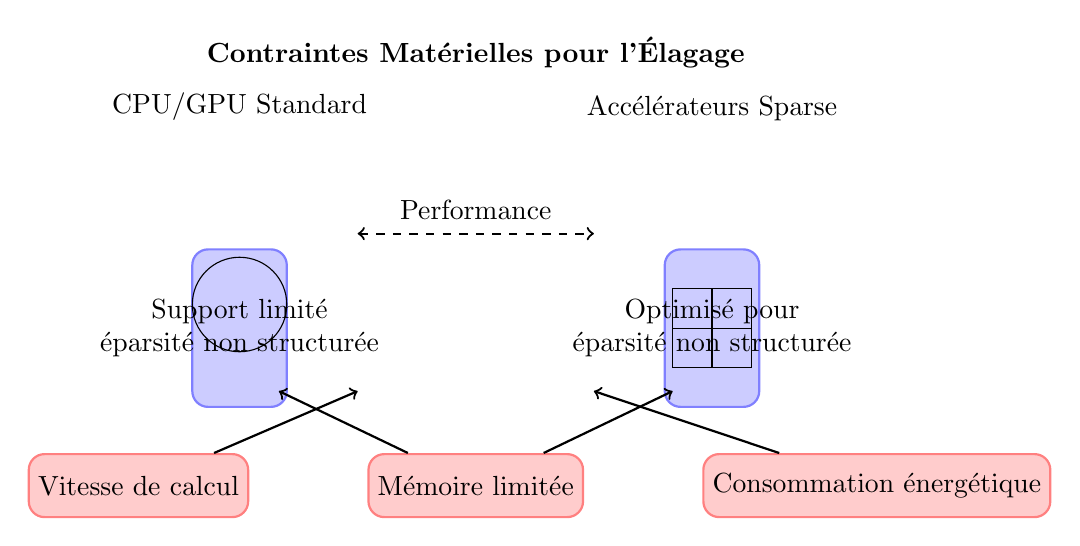
\begin{tikzpicture}[
    node distance=1.5cm,
    device/.style={rectangle, draw=blue!50, fill=blue!20, thick, minimum width=1.2cm, minimum height=2cm, rounded corners=0.2cm},
    constraint/.style={rectangle, draw=red!50, fill=red!20, thick, minimum width=2cm, minimum height=0.8cm, rounded corners=0.2cm}
]

% Title
\node at (0, 3.5) {\textbf{Contraintes Matérielles pour l'Élagage}};

% Standard hardware
\node[device] (cpu) at (-3, 0) {};
\node[above=of cpu] {CPU/GPU Standard};
\draw (-3, 0.3) circle (0.6cm);
\node at (-3, 0) {\shortstack{Support limité\\éparsité non structurée}};

% Specialized hardware
\node[device] (sparse) at (3, 0) {};
\node[above=of sparse] {Accélérateurs Sparse};
\draw (3, 0) rectangle (3.5, 0.5);
\draw (2.5, 0) rectangle (3, 0.5);
\draw (3, -0.5) rectangle (3.5, 0);
\draw (2.5, -0.5) rectangle (3, 0);
\node at (3, 0) {\shortstack{Optimisé pour\\éparsité non structurée}};

% Constraints
\node[constraint] (mem) at (0, -2) {Mémoire limitée};
\node[constraint, right=of mem] (power) {Consommation énergétique};
\node[constraint, left=of mem] (speed) {Vitesse de calcul};

% Arrows
\draw[->, thick] (mem) -- (-2.5, -0.8);
\draw[->, thick] (mem) -- (2.5, -0.8);
\draw[->, thick] (power) -- (1.5, -0.8);
\draw[->, thick] (speed) -- (-1.5, -0.8);

% Comparison
\draw[<->, thick, dashed] (-1.5, 1.2) -- (1.5, 1.2);
\node at (0, 1.5) {Performance};

\end{tikzpicture}
\end{document}